% =====================================================================
% Defense presentation — Specification-Driven Testing
% Πέτρος Ευάγγελος Τριανταφύλλης  (transliterated on slides — see note)
% Defense: Friday 19 June 2026, 16:30, University of the Aegean, Samos
% Target: 30 minutes, ~20 slides
% Closing visual: closed control loop (Kritikos [605])
% =====================================================================
\documentclass[10pt,aspectratio=169]{beamer}

\usepackage[utf8]{inputenc}
\usepackage[T1]{fontenc}
\usepackage{lmodern}
\usepackage{microtype}
\usepackage{tikz}
\usetikzlibrary{arrows.meta,positioning,shapes.geometric,fit,backgrounds,calc}
\usepackage{pifont}
\usepackage{listings}
\newcommand{\cmark}{\textcolor{green!60!black}{\ding{51}}}
\newcommand{\xmark}{\textcolor{red!70!black}{\ding{55}}}

% Note: slides are English; Greek names are transliterated to keep the
% pdflatex build simple. The thesis already carries the canonical Greek
% spellings on the title and signature pages.

% --- Colour palette ------------------------------------------------------
\definecolor{sdtblue}{HTML}{1F4E79}
\definecolor{sdtorange}{HTML}{D97706}
\definecolor{sdtred}{HTML}{B91C1C}
\definecolor{sdtgreen}{HTML}{166534}
\definecolor{sdtviolet}{HTML}{6B21A8}
\definecolor{sdtteal}{HTML}{0F766E}

% --- Theme ---------------------------------------------------------------
\usetheme{metropolis}
\setbeamertemplate{navigation symbols}{}
\setbeamertemplate{frame numbering}[fraction]
\setbeamercolor{title separator}{fg=sdtblue}
\setbeamercolor{progress bar}{fg=sdtblue}
\setbeamercolor{alerted text}{fg=sdtred}

% --- TikZ helper styles --------------------------------------------------
% IMPORTANT: We avoid parameterised styles (name/.style={... #1 ...})
% because they collide with metropolis's frame-template \iterate macro
% inside beamer frames. Instead, each colour gets a concrete style.
\tikzset{
  % Small rounded box, ~2.5cm wide
  bx blue/.style    = {rectangle, rounded corners=3pt, draw=sdtblue!70!black,
                       fill=sdtblue!12, minimum width=2.4cm, minimum height=0.9cm,
                       font=\scriptsize, align=center},
  bx orange/.style  = {rectangle, rounded corners=3pt, draw=sdtorange!70!black,
                       fill=sdtorange!12, minimum width=2.4cm, minimum height=0.9cm,
                       font=\scriptsize, align=center},
  bx red/.style     = {rectangle, rounded corners=3pt, draw=sdtred!70!black,
                       fill=sdtred!12, minimum width=2.4cm, minimum height=0.9cm,
                       font=\scriptsize, align=center},
  bx green/.style   = {rectangle, rounded corners=3pt, draw=sdtgreen!70!black,
                       fill=sdtgreen!12, minimum width=2.4cm, minimum height=0.9cm,
                       font=\scriptsize, align=center},
  bx violet/.style  = {rectangle, rounded corners=3pt, draw=sdtviolet!70!black,
                       fill=sdtviolet!12, minimum width=2.4cm, minimum height=0.9cm,
                       font=\scriptsize, align=center},
  bx teal/.style    = {rectangle, rounded corners=3pt, draw=sdtteal!70!black,
                       fill=sdtteal!12, minimum width=2.4cm, minimum height=0.9cm,
                       font=\scriptsize, align=center},
  % Narrow variants for the XSDLC child-resource grid (slide 10) where
  % 7 boxes need to fit in one row without overlapping.
  nbx blue/.style   = {rectangle, rounded corners=2pt, draw=sdtblue!70!black,
                       fill=sdtblue!12, minimum width=1.55cm, minimum height=0.65cm,
                       font=\tiny, align=center, inner sep=2pt},
  nbx teal/.style   = {rectangle, rounded corners=2pt, draw=sdtteal!70!black,
                       fill=sdtteal!12, minimum width=1.55cm, minimum height=0.65cm,
                       font=\tiny, align=center, inner sep=2pt},
  % Wide rounded box (for env/stage labels)
  wbx blue/.style   = {rectangle, rounded corners=5pt, draw=sdtblue!70!black,
                       fill=sdtblue!12, minimum width=2.8cm, minimum height=1.2cm,
                       font=\small\bfseries, align=center},
  wbx orange/.style = {rectangle, rounded corners=5pt, draw=sdtorange!70!black,
                       fill=sdtorange!12, minimum width=2.8cm, minimum height=1.2cm,
                       font=\small\bfseries, align=center},
  wbx red/.style    = {rectangle, rounded corners=5pt, draw=sdtred!70!black,
                       fill=sdtred!12, minimum width=2.8cm, minimum height=1.2cm,
                       font=\small\bfseries, align=center},
  wbx green/.style  = {rectangle, rounded corners=5pt, draw=sdtgreen!70!black,
                       fill=sdtgreen!12, minimum width=2.8cm, minimum height=1.2cm,
                       font=\small\bfseries, align=center},
  wbx violet/.style = {rectangle, rounded corners=5pt, draw=sdtviolet!70!black,
                       fill=sdtviolet!12, minimum width=2.8cm, minimum height=1.2cm,
                       font=\small\bfseries, align=center},
  wbx teal/.style   = {rectangle, rounded corners=5pt, draw=sdtteal!70!black,
                       fill=sdtteal!12, minimum width=2.8cm, minimum height=1.2cm,
                       font=\small\bfseries, align=center},
  % Axiom circle
  ax blue/.style    = {circle, draw=sdtblue!70!black, fill=sdtblue!15,
                       minimum size=2.4cm, align=center, font=\small\bfseries},
  ax orange/.style  = {circle, draw=sdtorange!70!black, fill=sdtorange!15,
                       minimum size=2.4cm, align=center, font=\small\bfseries},
  ax green/.style   = {circle, draw=sdtgreen!70!black, fill=sdtgreen!15,
                       minimum size=2.4cm, align=center, font=\small\bfseries},
  % Banner box (mode quadrants)
  banner blue/.style    = {rectangle, rounded corners=4pt, draw=sdtblue!70!black,
                           fill=sdtblue!12, minimum width=4.5cm, minimum height=1.5cm,
                           align=center, font=\small},
  banner orange/.style  = {rectangle, rounded corners=4pt, draw=sdtorange!70!black,
                           fill=sdtorange!12, minimum width=4.5cm, minimum height=1.5cm,
                           align=center, font=\small},
  banner teal/.style    = {rectangle, rounded corners=4pt, draw=sdtteal!70!black,
                           fill=sdtteal!12, minimum width=4.5cm, minimum height=1.5cm,
                           align=center, font=\small},
  banner violet/.style  = {rectangle, rounded corners=4pt, draw=sdtviolet!70!black,
                           fill=sdtviolet!12, minimum width=4.5cm, minimum height=1.5cm,
                           align=center, font=\small},
  % Repo box
  repo blue/.style    = {rectangle, rounded corners=4pt, draw=sdtblue!70!black,
                         fill=sdtblue!12, minimum width=4cm, minimum height=1.6cm,
                         align=center, font=\small},
  repo green/.style   = {rectangle, rounded corners=4pt, draw=sdtgreen!70!black,
                         fill=sdtgreen!12, minimum width=4cm, minimum height=1.6cm,
                         align=center, font=\small},
  % Gate cell (red)
  gate cell/.style   = {rectangle, rounded corners=3pt, draw=sdtred!70!black,
                        fill=sdtred!10, minimum width=2cm, minimum height=0.7cm,
                        font=\scriptsize, align=center},
  % Control-loop block (slide 19) — fixed colour set
  ctrl violet/.style = {rectangle, rounded corners=4pt, draw=sdtviolet!70!black,
                        fill=sdtviolet!12, minimum width=2.6cm, minimum height=1cm,
                        font=\small, align=center},
  ctrl teal/.style   = {rectangle, rounded corners=4pt, draw=sdtteal!70!black,
                        fill=sdtteal!12, minimum width=2.6cm, minimum height=1cm,
                        font=\small, align=center},
  ctrl orange/.style = {rectangle, rounded corners=4pt, draw=sdtorange!70!black,
                        fill=sdtorange!12, minimum width=2.6cm, minimum height=1cm,
                        font=\small, align=center},
  ctrl blue/.style   = {rectangle, rounded corners=4pt, draw=sdtblue!70!black,
                        fill=sdtblue!12, minimum width=2.6cm, minimum height=1cm,
                        font=\small, align=center},
  ctrl red/.style    = {rectangle, rounded corners=4pt, draw=sdtred!70!black,
                        fill=sdtred!12, minimum width=2.6cm, minimum height=1cm,
                        font=\small, align=center},
  sum node/.style    = {circle, draw=sdtred!70!black, fill=sdtred!10,
                        minimum size=0.7cm, font=\bfseries\large},
  % Tiny sstep (proc-vs-loop transition)
  sstep/.style        = {rectangle, rounded corners=2pt, draw=gray!50, fill=gray!10,
                        minimum width=2.6cm, minimum height=0.55cm,
                        font=\scriptsize, align=center},
  sstep violet/.style = {rectangle, rounded corners=2pt, draw=sdtviolet!70!black,
                        fill=sdtviolet!10, minimum width=2.6cm, minimum height=0.55cm,
                        font=\scriptsize, align=center},
  sstep red/.style    = {rectangle, rounded corners=2pt, draw=sdtred!70!black,
                        fill=sdtred!10, minimum width=2.6cm, minimum height=0.55cm,
                        font=\scriptsize, align=center},
  sstep teal/.style   = {rectangle, rounded corners=2pt, draw=sdtteal!70!black,
                        fill=sdtteal!10, minimum width=2.6cm, minimum height=0.55cm,
                        font=\scriptsize, align=center},
  sstep orange/.style = {rectangle, rounded corners=2pt, draw=sdtorange!70!black,
                        fill=sdtorange!12, minimum width=2.6cm, minimum height=0.55cm,
                        font=\scriptsize, align=center},
}

% --- Metadata ------------------------------------------------------------
\title{Specification-Driven Testing (SDT)}
\subtitle{A Conceptual Framework for Automated API Quality\\
Assurance in the GitOps Era}
\author{Petros Evangelos Triantafyllis}
\institute{University of the Aegean\\
Department of Information and Communication Systems Engineering\\[1ex]
Supervisor: Prof.\ Kyriakos Kritikos}
\date{Defense — Friday 19 June 2026, Samos}

% =====================================================================
\begin{document}
% =====================================================================

% --------- 1. Title -----------------------------------------------------
\begin{frame}[plain,noframenumbering]
  \titlepage
\end{frame}

% =====================================================================
% Act 1 — The problem (slides 2–5)
% =====================================================================

% --------- 2. The procedure today --------------------------------------
\begin{frame}{The procedure today: fragmented}

\begin{center}
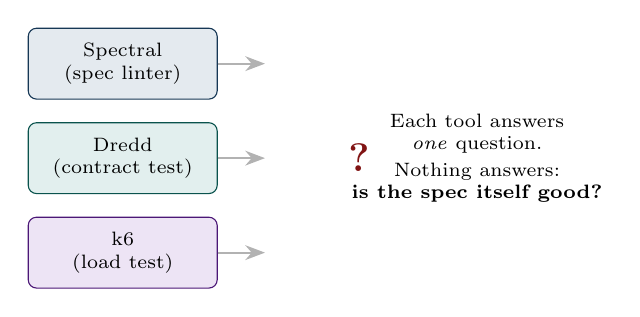
\begin{tikzpicture}[>={Stealth[length=2.5mm]}]
\node[bx blue]   (a) at (0,1.2)  {Spectral\\(spec linter)};
\node[bx teal]   (b) at (0,0)    {Dredd\\(contract test)};
\node[bx violet] (c) at (0,-1.2) {k6\\(load test)};

\node[font=\scriptsize, align=center] at (4.5,0)
  {Each tool answers\\\emph{one} question.\\[2pt]
   Nothing answers:\\\textbf{is the spec itself good?}};

\node[font=\Large\bfseries, text=sdtred!70!black] at (3.0,0) {?};

\draw[->,thick,gray!60] (a.east) -- ++(0.6,0);
\draw[->,thick,gray!60] (b.east) -- ++(0.6,0);
\draw[->,thick,gray!60] (c.east) -- ++(0.6,0);
\end{tikzpicture}
\end{center}

\vspace{0.5em}
\small
The specification is the only artefact common to dev, test, deploy, and
ops. Its quality bounds every downstream automation. Yet no existing
tool treats it as the primary object of validation.

\end{frame}

% --------- 3. Three failure modes --------------------------------------
\begin{frame}{Three failure modes}

\begin{columns}[t,onlytextwidth]

\column{0.32\textwidth}
\begin{center}
\textbf{\textcolor{sdtred}{Spec incomplete}}\\[1ex]
\xmark\\[1ex]
\footnotesize
Linters say it parses.\\
Consumers can't use it.\\
Agents can't act on it.
\end{center}

\column{0.32\textwidth}
\begin{center}
\textbf{\textcolor{sdtred}{Implementation drifts}}\\[1ex]
\xmark\\[1ex]
\footnotesize
Tests run too late.\\
Drift detected\\
after deployment.
\end{center}

\column{0.32\textwidth}
\begin{center}
\textbf{\textcolor{sdtred}{Pipeline is manual}}\\[1ex]
\xmark\\[1ex]
\footnotesize
ClickOps everywhere.\\
Gates assembled\\
by hand per app.
\end{center}

\end{columns}

\vspace{1em}
\begin{center}
\alert{One problem, three symptoms: the specification is not a
first-class artefact of the delivery pipeline.}
\end{center}

\end{frame}

% --------- 4. Research questions ---------------------------------------
\begin{frame}{Research questions}

\textbf{RQ1} — Can a conceptual framework demonstrate automated API
quality assurance \emph{without dedicated testers in the promotion path}?

\vspace{0.8em}
\textbf{RQ2} — To what extent can validation rules, test cases, and
quality gates be derived automatically from OpenAPI specifications?

\vspace{0.8em}
\textbf{RQ3} — How effectively does specification-driven QA integrate
into cloud-native GitOps pipelines?

\vspace{0.8em}
\textbf{RQ4} — Can quality-gated delivery pipelines be expressed as
\emph{Kubernetes-native ontological specifications} that operators and
autonomous agents can discover, inspect, and manage?

\end{frame}

% --------- 5. Contributions roadmap ------------------------------------
\begin{frame}{Three contributions — the deck's roadmap}

\begin{center}
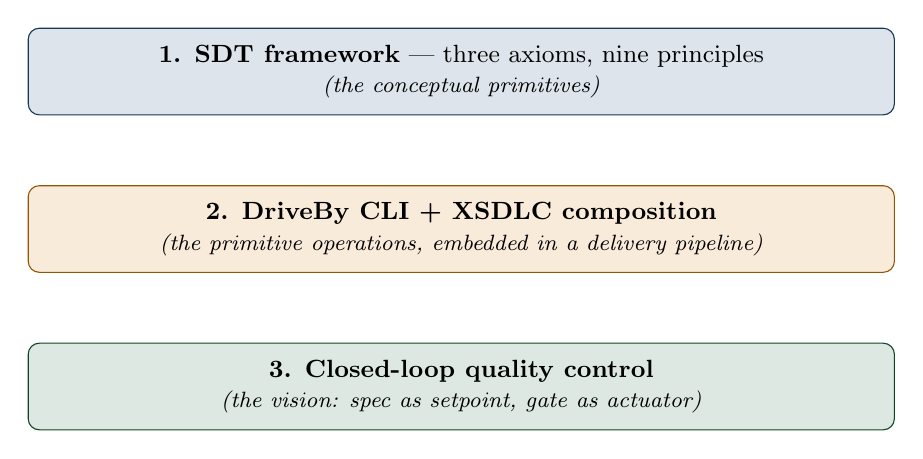
\begin{tikzpicture}
\node[rectangle, rounded corners=4pt, draw=sdtblue!70!black,
      fill=sdtblue!15, minimum width=11cm, minimum height=1.1cm,
      align=center, font=\small]
  (a) at (0,2)
  {\textbf{1. SDT framework} --- three axioms, nine principles\\
   \footnotesize\itshape (the conceptual primitives)};

\node[rectangle, rounded corners=4pt, draw=sdtorange!70!black,
      fill=sdtorange!15, minimum width=11cm, minimum height=1.1cm,
      align=center, font=\small]
  (b) at (0,0)
  {\textbf{2. DriveBy CLI + XSDLC composition}\\
   \footnotesize\itshape (the primitive operations, embedded in a delivery pipeline)};

\node[rectangle, rounded corners=4pt, draw=sdtgreen!70!black,
      fill=sdtgreen!15, minimum width=11cm, minimum height=1.1cm,
      align=center, font=\small]
  (c) at (0,-2)
  {\textbf{3. Closed-loop quality control}\\
   \footnotesize\itshape (the vision: spec as setpoint, gate as actuator)};
\end{tikzpicture}
\end{center}

\end{frame}

% =====================================================================
% Act 2 — Primitive ops (slides 6–14)
% =====================================================================

% --------- 6. The three axioms -----------------------------------------
\begin{frame}{The three axioms: the foundation}

\begin{columns}[c,onlytextwidth]

\column{0.45\textwidth}
\begin{center}
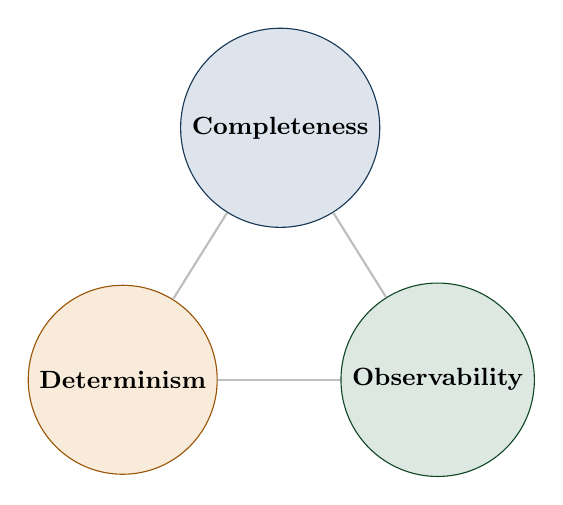
\begin{tikzpicture}
\node[ax blue]   (c) at (0,2.0)    {Completeness};
\node[ax orange] (d) at (-2.0,-1.2) {Determinism};
\node[ax green]  (o) at (2.0,-1.2)  {Observability};
\draw[thick, gray!50] (c) -- (d);
\draw[thick, gray!50] (d) -- (o);
\draw[thick, gray!50] (o) -- (c);
\end{tikzpicture}
\end{center}

\column{0.5\textwidth}
\footnotesize
\textbf{Completeness} — the specification must fully describe the API
contract.\\[1ex]

\textbf{Determinism} — same spec + same API $\Rightarrow$ same validation
result, every time.\\[1ex]

\textbf{Observability} — validation output must be structured,
quantifiable, machine-readable.\\[2ex]

\textit{The whole framework derives from these three.}

\end{columns}

\end{frame}

% --------- 7. The nine principles --------------------------------------
\begin{frame}{Nine principles: the primitive operations}

\begin{center}
\small
\begin{tabular}{@{}cll l@{}}
\textbf{ID} & \textbf{Principle} & \textbf{Axiom} & \textbf{Severity} \\
\hline
P001 & OpenAPI Compliance       & Completeness   & Critical \\
P002 & Documentation Quality    & Completeness   & Critical \\
P003 & Error Handling           & Completeness   & Critical \\
P004 & Schema Definitions       & Completeness   & Critical \\
P005 & Security Standards       & Observability  & Critical \\
\hline
P006 & Functional Testing       & Determinism    & Critical (runtime) \\
P007 & Performance Testing      & Observability  & Warning \\
\hline
P008 & Versioning Strategy      & Observability  & Warning \\
P009 & Test Readiness           & Determinism    & Warning \\
\end{tabular}
\end{center}

\vspace{1em}
\footnotesize
Each principle is an atomic check \emph{derivable from} the
specification. P001--P005 are static. P006--P007 require a running API.
P008--P009 are advisory.

\end{frame}

% --------- 8. Validation modes -----------------------------------------
\begin{frame}{Validation modes: composition primitives}

\begin{center}
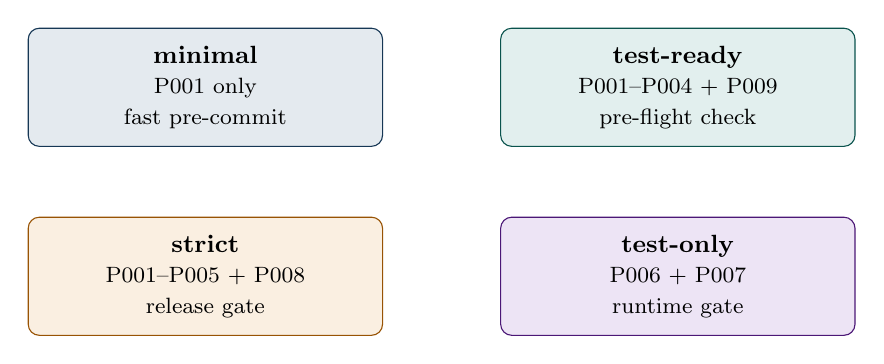
\begin{tikzpicture}
\node[banner blue]   (min) at (-3,1.2)  {\textbf{minimal}\\\footnotesize P001 only\\\footnotesize fast pre-commit};
\node[banner teal]   (tr)  at (3,1.2)   {\textbf{test-ready}\\\footnotesize P001--P004 + P009\\\footnotesize pre-flight check};
\node[banner orange] (st)  at (-3,-1.2) {\textbf{strict}\\\footnotesize P001--P005 + P008\\\footnotesize release gate};
\node[banner violet] (to)  at (3,-1.2)  {\textbf{test-only}\\\footnotesize P006 + P007\\\footnotesize runtime gate};
\end{tikzpicture}
\end{center}

\vspace{0.5em}
\footnotesize
\alert{Modes are not incremental.} \texttt{test-only} is
\emph{orthogonal} — it runs no static checks. Modes \emph{compose} in
the gate DAG (staging uses one combination, production another).

\end{frame}

% --------- 9. DriveBy CLI ----------------------------------------------
\begin{frame}{DriveBy: a single validator binary}

\begin{center}
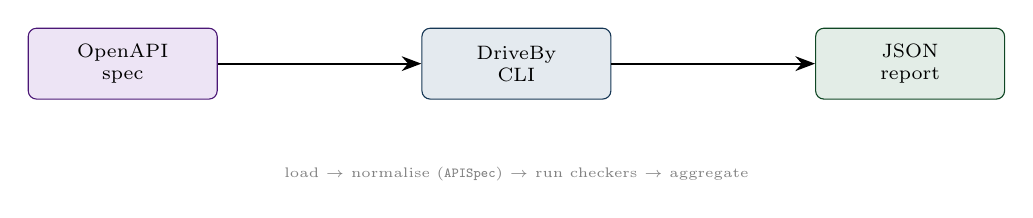
\begin{tikzpicture}[>={Stealth[length=2.5mm]}]
\node[bx violet] (spec)   at (-5,0) {OpenAPI\\spec};
\node[bx blue]   (cli)    at ( 0,0) {DriveBy\\CLI};
\node[bx green]  (report) at ( 5,0) {JSON\\report};

\draw[->,thick] (spec) -- (cli);
\draw[->,thick] (cli) -- (report);

\node[font=\tiny, text=gray, align=center] at (0,-1.4)
  {load $\rightarrow$ normalise (\texttt{APISpec}) $\rightarrow$ run checkers $\rightarrow$ aggregate};
\end{tikzpicture}
\end{center}

\vspace{0.7em}
\footnotesize
\begin{itemize}\setlength\itemsep{0.3em}
\item One Go binary; eleven internal packages; strict left-to-right
  dependency flow.
\item \texttt{APISpec} adapter abstracts OpenAPI~3.0.x, 3.1.0, and
  Swagger~2.0.
\item Report is a deterministic JSON document with severity-classified
  findings and per-principle \texttt{SuggestedFix} field.
\item JSON Schema for the report format is published at
  \texttt{driveby-cli/schemas/report.schema.json}.
\end{itemize}

\end{frame}

% --------- 10. XSDLC ---------------------------------------------------
\begin{frame}{XSDLC: from CLI tool to platform feature}

\begin{center}
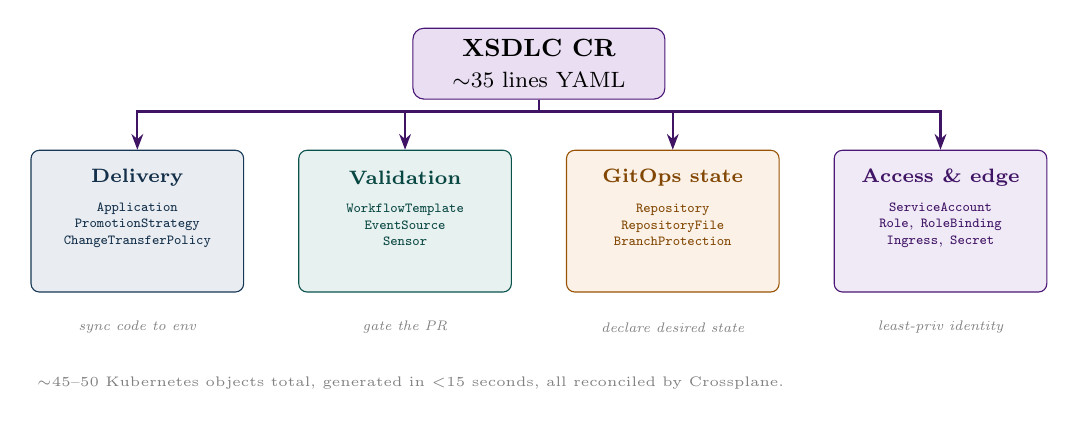
\begin{tikzpicture}[>={Stealth[length=2mm]}]

\node[rectangle, rounded corners=4pt, draw=sdtviolet!70!black,
      fill=sdtviolet!15, minimum width=3.2cm, minimum height=0.9cm,
      font=\small\bfseries, align=center]
  (xsdlc) at (0,2.0)
  {XSDLC CR\\\footnotesize\textnormal{$\sim$35 lines YAML}};

\node[rectangle, rounded corners=3pt, draw=sdtblue!70!black,
      fill=sdtblue!10, minimum width=2.7cm, minimum height=1.8cm,
      align=center]
  (g1) at (-5.1,0.0) {};
\node[font=\scriptsize\bfseries, text=sdtblue!60!black]
  at (-5.1,0.55) {Delivery};
\node[font=\tiny, align=center, text=sdtblue!60!black]
  at (-5.1,-0.05) {\texttt{Application}\\\texttt{PromotionStrategy}\\\texttt{ChangeTransferPolicy}};

\node[rectangle, rounded corners=3pt, draw=sdtteal!70!black,
      fill=sdtteal!10, minimum width=2.7cm, minimum height=1.8cm,
      align=center]
  (g2) at (-1.7,0.0) {};
\node[font=\scriptsize\bfseries, text=sdtteal!60!black]
  at (-1.7,0.55) {Validation};
\node[font=\tiny, align=center, text=sdtteal!60!black]
  at (-1.7,-0.05) {\texttt{WorkflowTemplate}\\\texttt{EventSource}\\\texttt{Sensor}};

\node[rectangle, rounded corners=3pt, draw=sdtorange!70!black,
      fill=sdtorange!10, minimum width=2.7cm, minimum height=1.8cm,
      align=center]
  (g3) at (1.7,0.0) {};
\node[font=\scriptsize\bfseries, text=sdtorange!60!black]
  at (1.7,0.55) {GitOps state};
\node[font=\tiny, align=center, text=sdtorange!60!black]
  at (1.7,-0.05) {\texttt{Repository}\\\texttt{RepositoryFile}\\\texttt{BranchProtection}};

\node[rectangle, rounded corners=3pt, draw=sdtviolet!70!black,
      fill=sdtviolet!10, minimum width=2.7cm, minimum height=1.8cm,
      align=center]
  (g4) at (5.1,0.0) {};
\node[font=\scriptsize\bfseries, text=sdtviolet!60!black]
  at (5.1,0.55) {Access \& edge};
\node[font=\tiny, align=center, text=sdtviolet!60!black]
  at (5.1,-0.05) {\texttt{ServiceAccount}\\\texttt{Role}, \texttt{RoleBinding}\\\texttt{Ingress}, \texttt{Secret}};

\node[font=\tiny\itshape, text=gray] at (-5.1,-1.35) {sync code to env};
\node[font=\tiny\itshape, text=gray] at (-1.7,-1.35) {gate the PR};
\node[font=\tiny\itshape, text=gray] at ( 1.7,-1.35) {declare desired state};
\node[font=\tiny\itshape, text=gray] at ( 5.1,-1.35) {least-priv identity};

\draw[->,thick,sdtviolet!60!black] (xsdlc.south) -- ++(0,-0.15) -| (g1.north);
\draw[->,thick,sdtviolet!60!black] (xsdlc.south) -- ++(0,-0.15) -| (g2.north);
\draw[->,thick,sdtviolet!60!black] (xsdlc.south) -- ++(0,-0.15) -| (g3.north);
\draw[->,thick,sdtviolet!60!black] (xsdlc.south) -- ++(0,-0.15) -| (g4.north);

\node[font=\tiny, text=gray, anchor=west] at (-6.5,-2.05)
  {$\sim$45--50 Kubernetes objects total, generated in $<$15 seconds, all reconciled by Crossplane.};
\end{tikzpicture}
\end{center}

\vspace{0.1em}
\footnotesize
\alert{The CR \emph{is} a specification.} One YAML file declares the
quality-gated delivery pipeline as a structurally typed Kubernetes
object --- the same idiom as the OpenAPI spec it validates.

\end{frame}

% --------- 10b. The XSDLC manifest in practice -------------------------
\begin{frame}[fragile]{What an XSDLC manifest actually looks like}

\vspace{-1.2em}
\begin{lstlisting}[basicstyle=\fontsize{6pt}{7pt}\ttfamily,
                   language=,frame=none,xleftmargin=0pt,aboveskip=0pt,belowskip=0pt]
apiVersion: driveby.io/v1alpha1
kind: XSDLC
metadata: { name: perfect-api }
spec:
  gitopsRepository: { owner: novelcore, name: perfect-api-gitops }
  apiConfig:        { port: 8000, openapiEndpoint: /openapi.json }
  validationDefaults: { validationMode: strict }
  environments:
    - { name: dev }
    - name: staging
      gate:
        checks:
          - type: validate-only
            validationConfig: { validationMode: test-ready }
          - type: functional-test
    - name: prod
      autoMerge: false
      gate:
        checks:
          - type: load-test
            loadTestConfig:
              concurrentUsers: 10
              testDuration:   "15s"
              maxLatencyP95:  "2s"
              minSuccessRate:  0.5
\end{lstlisting}

\tiny\itshape Real manifest --- \texttt{novelcore-perfect-api/xsdlc-perfect-api.yaml}.

\end{frame}

% --------- 11. Two-repo BYOCI ------------------------------------------
\begin{frame}{Two-repo model: the BYOCI boundary}

\begin{center}
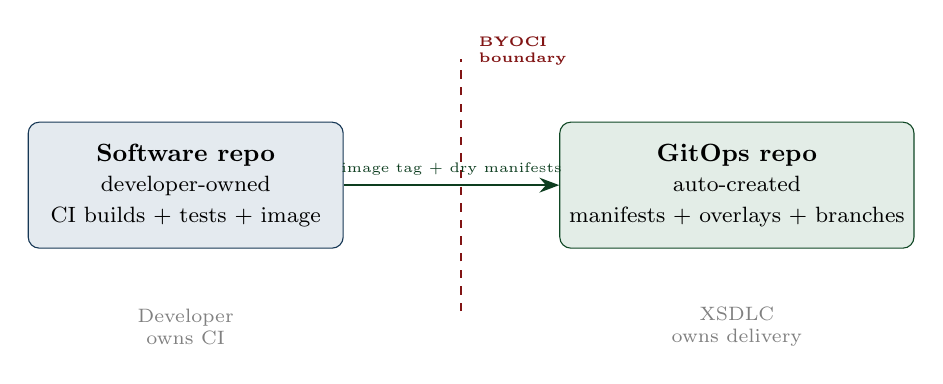
\begin{tikzpicture}[>={Stealth[length=2.5mm]}]
\node[repo blue]  (soft) at (-3.5,0) {\textbf{Software repo}\\\footnotesize developer-owned\\\footnotesize CI builds + tests + image};
\node[repo green] (gops) at ( 3.5,0) {\textbf{GitOps repo}\\\footnotesize auto-created\\\footnotesize manifests + overlays + branches};

\draw[dashed, thick, sdtred!70!black] (0,-1.6) -- (0,1.6);
\node[font=\tiny\bfseries, text=sdtred!70!black, anchor=west, align=left]
  at (0.1,1.7) {BYOCI\\boundary};

\node[font=\scriptsize, text=gray, align=center] at (-3.5,-1.8) {Developer\\owns CI};
\node[font=\scriptsize, text=gray, align=center] at ( 3.5,-1.8) {XSDLC\\owns delivery};

\draw[->,thick,sdtgreen!60!black] (soft.east) -- node[above,font=\tiny]{image tag + dry manifests} (gops.west);
\end{tikzpicture}
\end{center}

\vspace{0.4em}
\footnotesize
\textbf{Bring Your Own CI}: the developer's existing CI keeps building
and testing as before. XSDLC owns only what comes after the build ---
promotion, quality gating, environment management.

\end{frame}

% --------- 12. End-to-end gate procedure -------------------------------
\begin{frame}{The end-to-end gate procedure}

\begin{center}
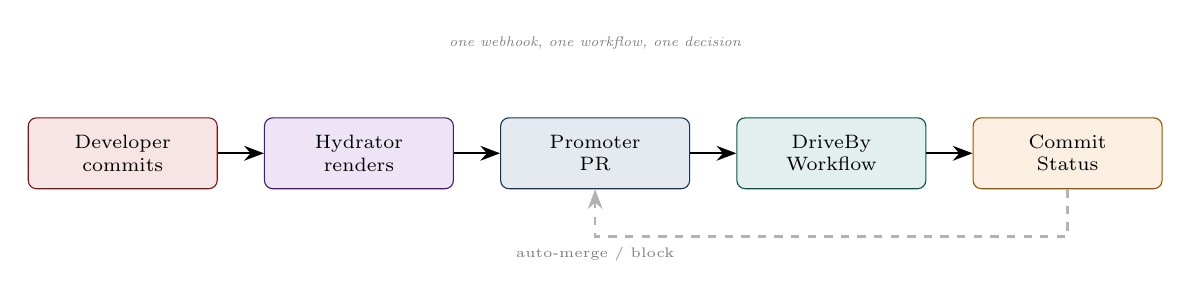
\begin{tikzpicture}[>={Stealth[length=2.5mm]}]
\node[bx red]    (push) at (-6,0)  {Developer\\commits};
\node[bx violet] (hyd)  at (-3,0)  {Hydrator\\renders};
\node[bx blue]   (pr)   at ( 0,0)  {Promoter\\PR};
\node[bx teal]   (gate) at ( 3,0)  {DriveBy\\Workflow};
\node[bx orange] (cs)   at ( 6,0)  {Commit\\Status};

\draw[->,thick] (push) -- (hyd);
\draw[->,thick] (hyd) -- (pr);
\draw[->,thick] (pr) -- (gate);
\draw[->,thick] (gate) -- (cs);

\draw[->,dashed,thick,gray!60] (cs.south) -- ++(0,-0.6) -| (pr.south)
  node[midway, below, font=\tiny, text=gray] {auto-merge / block};

\node[font=\tiny\itshape, text=gray] at (0,1.4)
  {one webhook, one workflow, one decision};
\end{tikzpicture}
\end{center}

\vspace{1em}
\footnotesize
\begin{itemize}\setlength\itemsep{0.3em}
\item Trigger is the \emph{promotion PR} that the Promoter opens.
\item DriveBy validates the \emph{source} environment (where the new
  code already runs), not the target.
\item Pass $\Rightarrow$ commit status success $\Rightarrow$ auto-merge
  $\Rightarrow$ ArgoCD syncs.
\item Fail $\Rightarrow$ commit status failure $\Rightarrow$ PR stays
  open $\Rightarrow$ developer iterates.
\end{itemize}

\end{frame}

% --------- 12b. Feedback: PR comment with beautified report ------------
\begin{frame}[fragile]{Feedback in the developer's natural habitat}

\footnotesize
The Workflow's exit handler posts the DriveBy report \emph{as a PR
comment} --- developers see precisely which principle failed and how
to fix it, on the very PR the Promoter just opened.

\vspace{0.5em}
\begin{center}
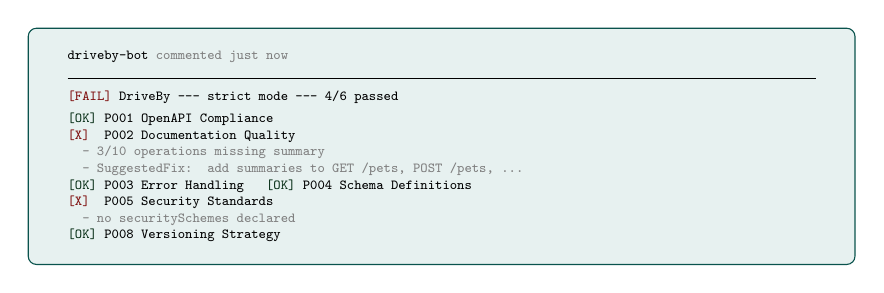
\begin{tikzpicture}[>={Stealth[length=2mm]}]
\node[rectangle, rounded corners=3pt, draw=sdtteal!70!black,
      fill=sdtteal!10, minimum width=10.5cm, minimum height=3.0cm,
      align=left, font=\tiny\ttfamily, inner sep=6pt]
  (pr) at (0,0)
  {\textbf{driveby-bot} \textcolor{gray}{commented just now} \\[1pt]
   \rule{9.5cm}{0.3pt} \\[2pt]
   \textbf{\textcolor{sdtred!70!black}{[FAIL]} DriveBy --- strict mode --- 4/6 passed} \\[2pt]
   \textcolor{sdtgreen!50!black}{[OK]} P001 OpenAPI Compliance \\
   \textcolor{sdtred!70!black}{[X]}~ P002 Documentation Quality \\
   \quad\textcolor{gray}{- 3/10 operations missing \texttt{summary}} \\
   \quad\textcolor{gray}{- SuggestedFix: add summaries to GET /pets, POST /pets, \ldots} \\
   \textcolor{sdtgreen!50!black}{[OK]} P003 Error Handling \quad
   \textcolor{sdtgreen!50!black}{[OK]} P004 Schema Definitions \\
   \textcolor{sdtred!70!black}{[X]}~ P005 Security Standards \\
   \quad\textcolor{gray}{- no \texttt{securitySchemes} declared} \\
   \textcolor{sdtgreen!50!black}{[OK]} P008 Versioning Strategy};
\end{tikzpicture}
\end{center}

\vspace{0.3em}
\tiny
\begin{itemize}\setlength\itemsep{0.15em}
\item Same JSON report, rendered as Markdown by the
  \texttt{comment-pr-failure} exit handler.
\item Commit status is the \emph{decision}; the PR comment is the
  \emph{explanation} --- and the \texttt{SuggestedFix} field makes the
  remediation actionable.
\end{itemize}

\end{frame}

% --------- 13. Multi-environment promotion -----------------------------
\begin{frame}{Multi-environment promotion}

\begin{center}
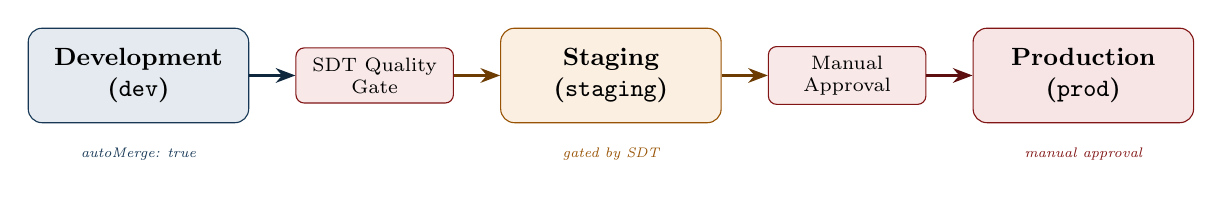
\begin{tikzpicture}[>={Stealth[length=2.5mm]}]
\node[wbx blue]   (dev)     at (0,0)  {Development\\(\texttt{dev})};
\node[gate cell]  (g1)      at (3,0)  {SDT Quality\\Gate};
\node[wbx orange] (staging) at (6,0)  {Staging\\(\texttt{staging})};
\node[gate cell]  (g2)      at (9,0)  {Manual\\Approval};
\node[wbx red]    (prod)    at (12,0) {Production\\(\texttt{prod})};

\draw[->,thick,sdtblue!50!black]   (dev)     -- (g1);
\draw[->,thick,sdtorange!50!black] (g1)      -- (staging);
\draw[->,thick,sdtorange!50!black] (staging) -- (g2);
\draw[->,thick,sdtred!50!black]    (g2)      -- (prod);

\node[font=\tiny\itshape, text=sdtblue!70!black]   at (0,-1.0) {autoMerge: true};
\node[font=\tiny\itshape, text=sdtorange!70!black] at (6,-1.0) {gated by SDT};
\node[font=\tiny\itshape, text=sdtred!70!black]    at (12,-1.0) {manual approval};
\end{tikzpicture}
\end{center}

\vspace{1em}
\footnotesize
The same gate template instantiated per environment, with different
modes per stage. Three is the minimum useful environment count; the
framework supports any \emph{N $\geq$ 2}.

\end{frame}

% --------- 14. 59 atomic checks ----------------------------------------
\begin{frame}{What's being measured: 59 atomic checks}

\begin{center}
\small
\begin{tabular}{@{}lcr@{\hskip 2em}lcr@{}}
\textbf{Principle} & & \textbf{Checks} & \textbf{Principle} & & \textbf{Checks} \\
\hline
P001 OpenAPI Compliance      & & 7  & P005 Security Standards   & & 7 \\
P002 Documentation Quality   & & 10 & P006 Functional Testing   & & 7 \\
P003 Error Handling          & & 7  & P008 Versioning Strategy  & & 7 \\
P004 Schema Definitions      & & 10 & P009 Test Readiness       & & 4 \\
\hline
\multicolumn{6}{r}{\textbf{Total: 59 atomic, spec-derivable checks}}
\end{tabular}
\end{center}

\vspace{1em}
\footnotesize
\begin{itemize}\setlength\itemsep{0.3em}
\item Each check is a pure function on the parsed \texttt{APISpec} ---
  no side effects, no environment dependencies.
\item Each emits a structured result with \texttt{name},
  \texttt{passed}, \texttt{message}, \texttt{suggestedFix}.
\item Aggregated into per-principle pass/fail and per-report severity
  count.
\item \alert{Zero manually authored test cases.}
\end{itemize}

\end{frame}

% =====================================================================
% Act 3 — Evidence + the closed loop (slides 15–20)
% =====================================================================

% --------- 15. Three evaluation arms -----------------------------------
\begin{frame}{Evaluation: three arms}

\begin{center}
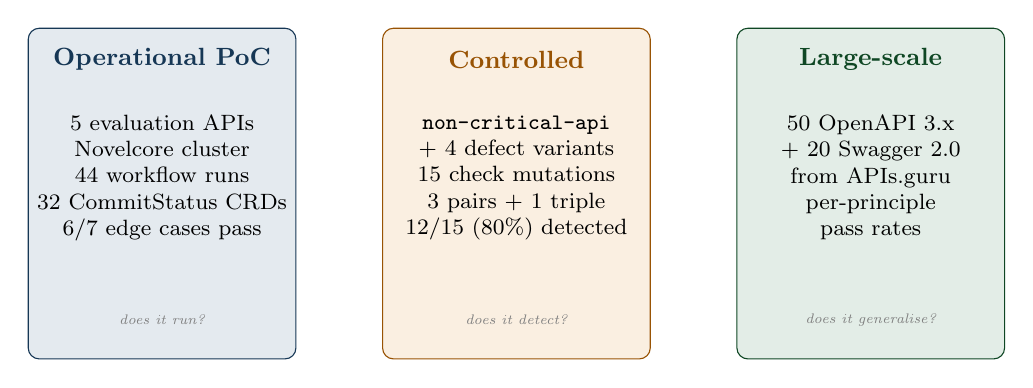
\begin{tikzpicture}
\node[rectangle, rounded corners=4pt, draw=sdtblue!70!black,
      fill=sdtblue!12, minimum width=3.4cm, minimum height=4.2cm,
      align=center] (a) at (-4.5,0) {};
\node[rectangle, rounded corners=4pt, draw=sdtorange!70!black,
      fill=sdtorange!12, minimum width=3.4cm, minimum height=4.2cm,
      align=center] (b) at ( 0,0) {};
\node[rectangle, rounded corners=4pt, draw=sdtgreen!70!black,
      fill=sdtgreen!12, minimum width=3.4cm, minimum height=4.2cm,
      align=center] (c) at ( 4.5,0) {};

\node[font=\small\bfseries, text=sdtblue!70!black]   at (-4.5,1.7) {Operational PoC};
\node[font=\small\bfseries, text=sdtorange!70!black] at ( 0,1.7)   {Controlled};
\node[font=\small\bfseries, text=sdtgreen!70!black]  at ( 4.5,1.7) {Large-scale};

\node[align=center, font=\footnotesize] at (-4.5, 0.2)
  {5 evaluation APIs\\Novelcore cluster\\44 workflow runs\\32 CommitStatus CRDs\\6/7 edge cases pass};

\node[align=center, font=\footnotesize] at ( 0, 0.2)
  {\texttt{non-critical-api}\\+ 4 defect variants\\15 check mutations\\3 pairs + 1 triple\\12/15 (80\%) detected};

\node[align=center, font=\footnotesize] at ( 4.5, 0.2)
  {50 OpenAPI 3.x\\+ 20 Swagger 2.0\\from APIs.guru\\per-principle\\pass rates};

\node[font=\tiny\itshape, text=gray] at (-4.5,-1.6) {does it run?};
\node[font=\tiny\itshape, text=gray] at ( 0,-1.6)   {does it detect?};
\node[font=\tiny\itshape, text=gray] at ( 4.5,-1.6) {does it generalise?};
\end{tikzpicture}
\end{center}

\end{frame}

% --------- 16. The 84% finding -----------------------------------------
\begin{frame}{Large-scale evaluation: a systemic quality gap}

\begin{center}
\small
\textbf{APIs.guru, strict mode}\\[0.5ex]
\footnotesize 50 OpenAPI 3.x + 20 Swagger 2.0 = 70 distinct providers
\end{center}

\vspace{0.5em}
\begin{center}
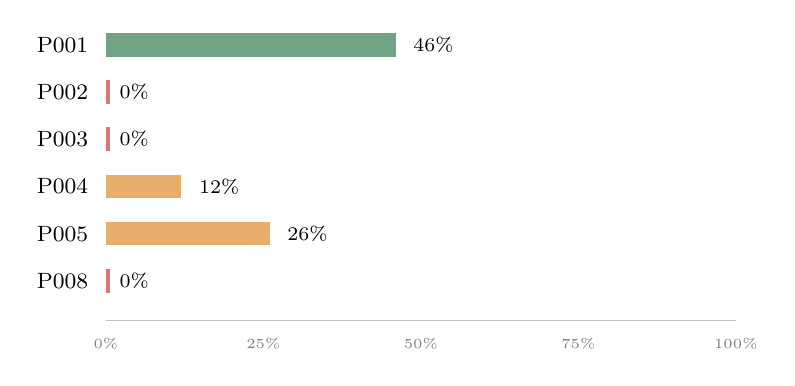
\begin{tikzpicture}
\node[font=\footnotesize, anchor=east] at (1.5, 2.0)  {P001};
\node[font=\footnotesize, anchor=east] at (1.5, 1.4)  {P002};
\node[font=\footnotesize, anchor=east] at (1.5, 0.8)  {P003};
\node[font=\footnotesize, anchor=east] at (1.5, 0.2)  {P004};
\node[font=\footnotesize, anchor=east] at (1.5,-0.4)  {P005};
\node[font=\footnotesize, anchor=east] at (1.5,-1.0)  {P008};

\fill[sdtgreen!60]  (1.6, 1.85) rectangle (1.6+46*0.08, 2.15);
\fill[sdtred!60]    (1.6, 1.25) rectangle (1.6+ 0.05    , 1.55);
\fill[sdtred!60]    (1.6, 0.65) rectangle (1.6+ 0.05    , 0.95);
\fill[sdtorange!60] (1.6, 0.05) rectangle (1.6+12*0.08, 0.35);
\fill[sdtorange!60] (1.6,-0.55) rectangle (1.6+26*0.08,-0.25);
\fill[sdtred!60]    (1.6,-1.15) rectangle (1.6+ 0.05    ,-0.85);

\node[font=\scriptsize, anchor=west] at (1.6+46*0.08+0.1, 2.0)  {46\%};
\node[font=\scriptsize, anchor=west] at (1.65, 1.4)  {0\%};
\node[font=\scriptsize, anchor=west] at (1.65, 0.8)  {0\%};
\node[font=\scriptsize, anchor=west] at (1.6+12*0.08+0.1, 0.2)  {12\%};
\node[font=\scriptsize, anchor=west] at (1.6+26*0.08+0.1,-0.4)  {26\%};
\node[font=\scriptsize, anchor=west] at (1.65,-1.0)  {0\%};

\draw[gray!50, thin] (1.6,-1.5) -- (9.6,-1.5);
\node[font=\tiny, text=gray, anchor=north] at (1.6, -1.6) {0\%};
\node[font=\tiny, text=gray, anchor=north] at (3.6, -1.6) {25\%};
\node[font=\tiny, text=gray, anchor=north] at (5.6, -1.6) {50\%};
\node[font=\tiny, text=gray, anchor=north] at (7.6, -1.6) {75\%};
\node[font=\tiny, text=gray, anchor=north] at (9.6, -1.6) {100\%};
\end{tikzpicture}
\end{center}

\vspace{0.5em}
\begin{center}
\alert{\textbf{84\% of public APIs score 1/6 or worse in strict mode.\\
No API in the sample passes more than 2 of the 6 evaluated
principles.}}
\end{center}

\end{frame}

% --------- 17. Agent-feedback experiment -------------------------------
\begin{frame}{Agent-feedback experiment: 1/6 $\rightarrow$ 4/6}

\begin{columns}[c,onlytextwidth]

\column{0.45\textwidth}
\begin{center}
\textbf{Swagger Petstore (baseline)}\\[1ex]
\footnotesize
\begin{tabular}{ll}
P001 & \cmark \\
P002 & \xmark \\
P003 & \xmark \\
P004 & \xmark \\
P005 & \xmark \\
P008 & \xmark \\
\hline
\textbf{1/6} &
\end{tabular}
\end{center}

\column{0.1\textwidth}
\begin{center}\Large $\rightarrow$\end{center}

\column{0.45\textwidth}
\begin{center}
\textbf{After one agent iteration}\\[1ex]
\footnotesize
\begin{tabular}{ll}
P001 & \cmark \\
P002 & \cmark \\
P003 & \cmark \\
P004 & \cmark \\
P005 & \xmark \\
P008 & \xmark \\
\hline
\textbf{4/6} & \footnotesize\itshape (+300\%)
\end{tabular}
\end{center}

\end{columns}

\vspace{1.5em}
\footnotesize
\begin{itemize}\setlength\itemsep{0.3em}
\item AI coding agent received \emph{only} the DriveBy JSON report.
\item No prompt about what to fix. No example revisions.
\item Agent autonomously edited the spec; re-validation gave 4/6.
\end{itemize}

\vspace{0.5em}
\begin{center}
\alert{SDT's structured output is sufficient feedback for autonomous
specification improvement.}
\end{center}

\end{frame}

% --------- 18. Procedure → control loop --------------------------------
\begin{frame}{From procedure to control loop}

\begin{columns}[T,onlytextwidth]

\column{0.45\textwidth}
\begin{center}
\textbf{Procedure} (Acts 1--2)\\[0.8em]
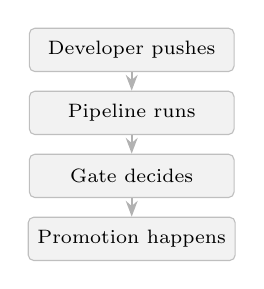
\begin{tikzpicture}[>={Stealth[length=2mm]}]
\node[sstep] (a) at (0, 1.6) {Developer pushes};
\node[sstep] (b) at (0, 0.8) {Pipeline runs};
\node[sstep] (c) at (0, 0.0) {Gate decides};
\node[sstep] (d) at (0,-0.8) {Promotion happens};
\draw[->,thick,gray!60] (a) -- (b);
\draw[->,thick,gray!60] (b) -- (c);
\draw[->,thick,gray!60] (c) -- (d);
\end{tikzpicture}
\end{center}

\column{0.1\textwidth}
\begin{center}
\vspace{1.5em}\Large \textcolor{sdtblue}{$\Rightarrow$}
\end{center}

\column{0.45\textwidth}
\begin{center}
\textbf{Closed loop} (Act 3)\\[0.8em]
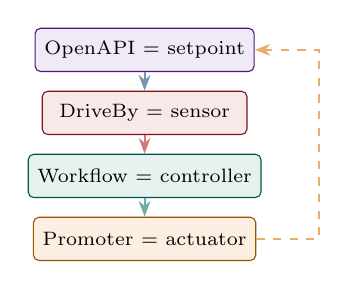
\begin{tikzpicture}[>={Stealth[length=2mm]}]
\node[sstep violet] (sp) at (0, 1.6) {OpenAPI = setpoint};
\node[sstep red]    (se) at (0, 0.8) {DriveBy = sensor};
\node[sstep teal]   (co) at (0, 0.0) {Workflow = controller};
\node[sstep orange] (ac) at (0,-0.8) {Promoter = actuator};
\draw[->,thick,sdtblue!60] (sp) -- (se);
\draw[->,thick,sdtred!60]  (se) -- (co);
\draw[->,thick,sdtteal!60] (co) -- (ac);
\draw[->,dashed,thick,sdtorange!60] (ac.east) -- ++(0.8,0) |- (sp.east);
\end{tikzpicture}
\end{center}

\end{columns}

\vspace{1.5em}
\begin{center}
\footnotesize
\alert{The pipeline is not just a procedure. It is a closed-loop
control system, with the specification as the setpoint and the gate as
the actuator.}
\end{center}

\end{frame}

% --------- 19. Closed control loop (centrepiece) -----------------------
\begin{frame}{Closed control loop: the vision}

\begin{center}
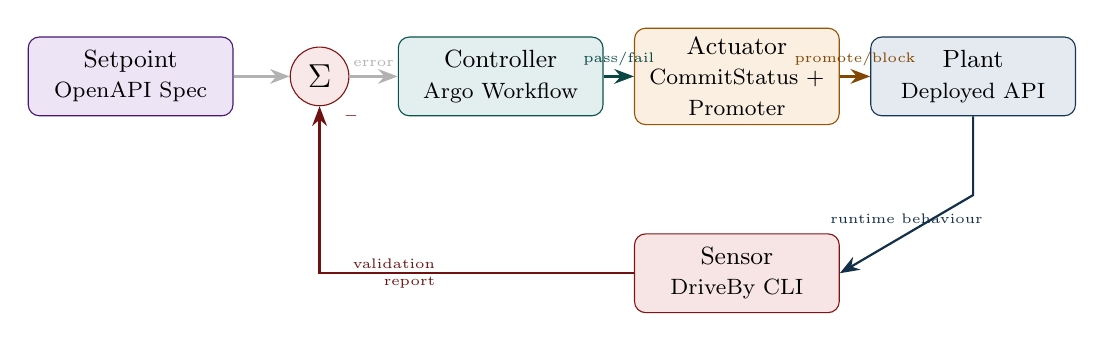
\begin{tikzpicture}[>={Stealth[length=2.5mm]}]
\node[ctrl violet] (setpoint)   at (0,0)    {Setpoint\\\footnotesize OpenAPI Spec};
\node[sum node]    (sum)        at (2.4,0)  {$\Sigma$};
\node[ctrl teal]   (controller) at (4.7,0)  {Controller\\\footnotesize Argo Workflow};
\node[ctrl orange] (actuator)   at (7.7,0)  {Actuator\\\footnotesize CommitStatus +\\\footnotesize Promoter};
\node[ctrl blue]   (plant)      at (10.7,0) {Plant\\\footnotesize Deployed API};
\node[ctrl red]    (sensor)     at (7.7,-2.5) {Sensor\\\footnotesize DriveBy CLI};

\draw[->,thick,gray!60]    (setpoint)   -- (sum);
\draw[->,thick,gray!60]    (sum)        -- node[above,font=\tiny]{error} (controller);
\draw[->,thick,sdtteal!60!black]   (controller) -- node[above,font=\tiny]{pass/fail} (actuator);
\draw[->,thick,sdtorange!60!black] (actuator)   -- node[above,font=\tiny]{promote/block} (plant);
\draw[->,thick,sdtblue!60!black]   (plant.south) -- ++(0,-1) -- node[above,font=\tiny]{runtime behaviour} (sensor.east);
\draw[->,thick,sdtred!60!black]    (sensor.west) -| node[left,font=\tiny,pos=0.3,align=right]{validation\\report} (sum.south);

\node[font=\tiny\bfseries, text=sdtred!70!black] at (2.8,-0.5) {$-$};
\end{tikzpicture}
\end{center}

\vspace{0.5em}
\footnotesize
\begin{itemize}\setlength\itemsep{0.2em}
\item Supervisor's review \emph{[605]}: ``\emph{Please highlight this as
  the main vision: a closed control loop, potentially with multiple
  levels, operating across clusters\ldots\ enabling system
  self-adjustment.}''
\item The thesis delivers the \alert{inner loop}.
\item The outer loops --- adaptive thresholds, agent-driven remediation,
  multi-cluster orchestration --- are the natural research
  continuation.
\end{itemize}

\end{frame}

% --------- 20. Closing -------------------------------------------------
\begin{frame}{Contributions, limitations, future work}

\begin{columns}[T,onlytextwidth]

\column{0.33\textwidth}
\textbf{Contributions}\\[0.5em]
\footnotesize
\begin{enumerate}\setlength\itemsep{0.2em}
  \item SDT framework
  \item DriveBy CLI
  \item XSDLC composition
  \item Empirical evidence
  \item Agent-feedback proof
  \item Agent-driven dev method
\end{enumerate}

\column{0.33\textwidth}
\textbf{Limitations}\\[0.5em]
\footnotesize
\begin{itemize}\setlength\itemsep{0.2em}
  \item P006/P007 wrappers pending
  \item Single-cluster PoC
  \item OpenAPI-only today
  \item Binary pass/fail scoring
\end{itemize}

\column{0.33\textwidth}
\textbf{Future work}\\[0.5em]
\footnotesize
\begin{itemize}\setlength\itemsep{0.2em}
  \item Adaptive thresholds
  \item Risk-based scoring
  \item Agent-driven remediation
  \item Multi-format adapters
  \item Multi-cluster control
  \item \emph{Outer control loops}
\end{itemize}

\end{columns}

\vspace{2em}
\begin{center}
\Large\textbf{Thank you.}\\[0.6em]
\normalsize Questions?
\end{center}

\end{frame}

\end{document}
